%%%%%%%%%%%%%%%%%%%%%%%%%%%%%%%%%%%%%%%%%
% Stylish Article
% LaTeX Template
% Version 2.2 (2020-10-22)
%
% This template has been downloaded from:
% http://www.LaTeXTemplates.com
%
% Original author:
% Mathias Legrand (legrand.mathias@gmail.com) 
% With extensive modifications by:
% Vel (vel@latextemplates.com)
% Jacqueline Näther (jnaether@uni-osnabrueck.com)
% Fabian Imkenberg (fimkenberg@uni-osnabrueck.com)
%
% License:
% CC BY-NC-SA 3.0 (http://creativecommons.org/licenses/by-nc-sa/3.0/)
%
%%%%%%%%%%%%%%%%%%%%%%%%%%%%%%%%%%%%%%%%%

%----------------------------------------------------------------------------------------
%	PACKAGES AND OTHER DOCUMENT CONFIGURATIONS
%----------------------------------------------------------------------------------------

\documentclass[fleqn,10pt]{SelfArx} % Document font size and equations flushed left

\usepackage[english]{babel} % Specify a different language here - english by default

\usepackage{lipsum} % Required to insert dummy text. To be removed otherwise

\usepackage[nolist]{acronym}	% [nolist]: Acronym list should not be print out.

\usepackage{listings}	% Required to insert lstlisting environment for code.

\usepackage{makecell}	% For manual line breaks in tables

%----------------------------------------------------------------------------------------
%	COLUMNS
%----------------------------------------------------------------------------------------

\setlength{\columnsep}{0.55cm} % Distance between the two columns of text
\setlength{\fboxrule}{0.75pt} % Width of the border around the abstract

%----------------------------------------------------------------------------------------
%	COLORS
%----------------------------------------------------------------------------------------

\definecolor{color1}{RGB}{172,06,52} % Corporate Design Colour of University of Osnabrueck
\definecolor{color2}{RGB}{207,208,209} % Corporate Design Colour of University of Osnabrueck
\definecolor{color3}{RGB}{251,185,0} % Corporate Design Colour of University of Osnabrueck
\definecolor{codegreen}{rgb}{0,0.6,0}
\definecolor{codegray}{rgb}{0.5,0.5,0.5}
\definecolor{codepurple}{rgb}{0.58,0,0.82}
\definecolor{backcolour}{rgb}{0.95,0.95,0.92}

%----------------------------------------------------------------------------------------
%	LISTING STYLE
%----------------------------------------------------------------------------------------

\lstdefinestyle{mystyle}{
    backgroundcolor=\color{backcolour},   
    commentstyle=\color{codegreen},
    keywordstyle=\color{magenta},
    numberstyle=\tiny\color{codegray},
    stringstyle=\color{codepurple},
    basicstyle=\ttfamily\footnotesize,
    breakatwhitespace=false,         
    breaklines=true,                 
    captionpos=b,                    
    keepspaces=true,                 
    numbers=left,                    
    numbersep=5pt,                  
    showspaces=false,                
    showstringspaces=false,
    showtabs=false,                  
    tabsize=2
}

\lstset{style=mystyle}

%----------------------------------------------------------------------------------------
%	HYPERLINKS
%----------------------------------------------------------------------------------------

\usepackage{hyperref} % Required for hyperlinks

\hypersetup{
	hidelinks,
	colorlinks,
	breaklinks=true,
	urlcolor=color3,
	citecolor=color1,
	linkcolor=color1,
	bookmarksopen=false,
	pdftitle={Title},
	pdfauthor={Author},
}

%----------------------------------------------------------------------------------------
%	ARTICLE INFORMATION
%----------------------------------------------------------------------------------------

\JournalInfo{
\includegraphics[width=0.3\linewidth]{logo_uni}}
\Archive{} %!!NEEDED, otherwise \tableofcontent error, is for Additional notes below university logo (e.g. copyright, DOI, review/research article)

\PaperTitle{Reimplementation of a Cycle-Consistent Adversarial Network for unpaired Image-to-Image Translation}

\Authors{Fabian Imkenberg, Jacqueline Naether}

\Keywords{CycleGAN --- Unpaired Image-to-Image Translation --- Keyword3} 
\newcommand{\keywordname}{Keywords} % Defines the keywords heading name

%----------------------------------------------------------------------------------------
%	ABSTRACT
%----------------------------------------------------------------------------------------

\Abstract{Lorem ipsum dolor sit amet, consectetuer adipiscing elit. Ut purus elit, vestibulum ut, placerat ac, adipiscing vitae, felis. Curabitur dictum gravida mauris. Nam arcu libero, nonummy eget, consectetuer id, vulputate a, magna. Donec vehicula augue eu neque. Pellentesque habitant morbi tristique senectus et netus et malesuada fames ac turpis egestas. Mauris ut leo. Cras viverra metus rhoncus sem. Nulla et lectus vestibulum urna fringilla ultrices. Phasellus eu tellus sit amet tortor gravida placerat. Integer sapien est, iaculis in, pretium quis, viverra ac, nunc. Praesent eget sem vel leo ultrices bibendum. Aenean faucibus. Morbi dolor nulla, malesuada eu, pulvinar at, mollis ac, nulla. Curabitur auctor semper nulla. Donec varius orci eget risus. Duis nibh mi, congue eu, accumsan eleifend, sagittis quis, diam. Duis eget orci sit amet orci dignissim rutrum.}

%----------------------------------------------------------------------------------------

\begin{document}
\maketitle
\tableofcontents
\thispagestyle{empty} % Removes page numbering from the first page

%----------------------------------------------------------------------------------------
%	ARTICLE CONTENTS
%----------------------------------------------------------------------------------------

\section*{Introduction}
\addcontentsline{toc}{section}{Introduction}
As the basis of our project, we studied the paper \textit{Unpaired Image-to-Image Translation using Cycle-Consistent Adversarial Networks} from the \ac{BAIR} laboratory. The aim of the paper is to change different information in images. The developed network creates a new generated image based on an existing input image. Three different types of generated images are presented in this paper. A translation of a photograph to a painting by Monet, zebras to horses, and summer to winter and vice versa. The paper complements what has been learned in the module \ac{IANNWTF} by two essential building blocks, which basically depend on each other.~\cite{image-to-image-ccan}

Until now, training data was mostly available in input-output pairs. This means that in the example translation summer to winter, for each photo of a location in summer there also exists a photo of the same location in winter. Thus, the network previously learned translation using complete individual examples. In the case of the paper, however, a network is developed that is trained based on two domains. As training input, the network is fed a domain of, for example, summer images. The training output then contains a domain of winter images. The network learns the different properties of summer and winter based on these image domains.~\cite{image-to-image-ccan}

As a second building block, the simple \ac{GAN} as presented in \ac{IANNWTF} is extended into a so-called Cycle-\ac{GAN}. The name is based on the use of the Cycle Consistency Loss in the training phase. We reimplemented and tested such a Cycle-\ac{GAN} based on the paper.~\cite{image-to-image-ccan}

%------------------------------------------------

\section{Methods}

As a transfer performance, our goal is not to teach our network the same translation as described in the paper.  Therefore, we decided to optimize our network to perform a translation from apple images to orange images and vice versa. For this, we had to select a suitable dataset, as well as to work out the methodological basics of the network architecture from the paper. In the following, these basics will be explained.

\subsection{Architectures}
As the basis of the network architecture, the \ac{GAN} already known through the \ac{IANNWTF} module is extended to the Cycle-\ac{GAN} known through the paper \cite{image-to-image-ccan}.

\paragraph{\acl{GAN}s} basically exist out of two neural networks, which more or less battle against each other, the \textit{Generator} and \textit{Discriminator}. The Generator takes the input and generates a fake image out of it, while the Discriminator tries to discriminate between generated and true images. Both parts of the network are trained individually from each other. The loss used in training is the adversarial loss.~\cite{Introduction-to-Cycle-GANs, GAN-Courseware}

\paragraph{Cycle-\ac{GAN}s} extend this concept, in terms of unpaired image-to-image translation. As mentioned in the introduction, the chosen paper uses domains of input \textit{D\textsubscript{x}} and output images \textit{D\textsubscript{y}}. The Generator is trained two main functions. Generating images from domain \textit{D\textsubscript{x}} to images of domain \textit{D\textsubscript{y}} ($G: X \rightarrow Y$) and vice versa ($F: Y \rightarrow X$). This principle is shown in \autoref{fig:mappingFunctions}.~\cite{image-to-image-ccan}

\begin{figure} \centering 
% Using \begin{figure*} makes the figure take up the entire width of the page
	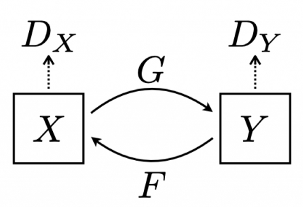
\includegraphics[width=0.8\linewidth]{mappingFunctions}
	\caption{Mapping functions of the Cycle-\ac{GAN}~\cite{image-to-image-ccan}}
	\label{fig:mappingFunctions}
\end{figure}

On the basis of this it becomes clear that a simple back and forward translation can lead to the fact that the back translation does not refer to exactly the original input image, but to another image within the input image domain. This is where the cycle consistency loss comes into play. This one is used in addition to the adversarial loss so that the network learns to return to the original image during a back and forward translation. The cycle consistency losses for the two mapping functions are shown in the \autoref{fig:cycleConsistencyLoss}.~\cite{image-to-image-ccan}

\begin{figure*}[htb] \centering 
% Using \begin{figure*} makes the figure take up the entire width of the page
	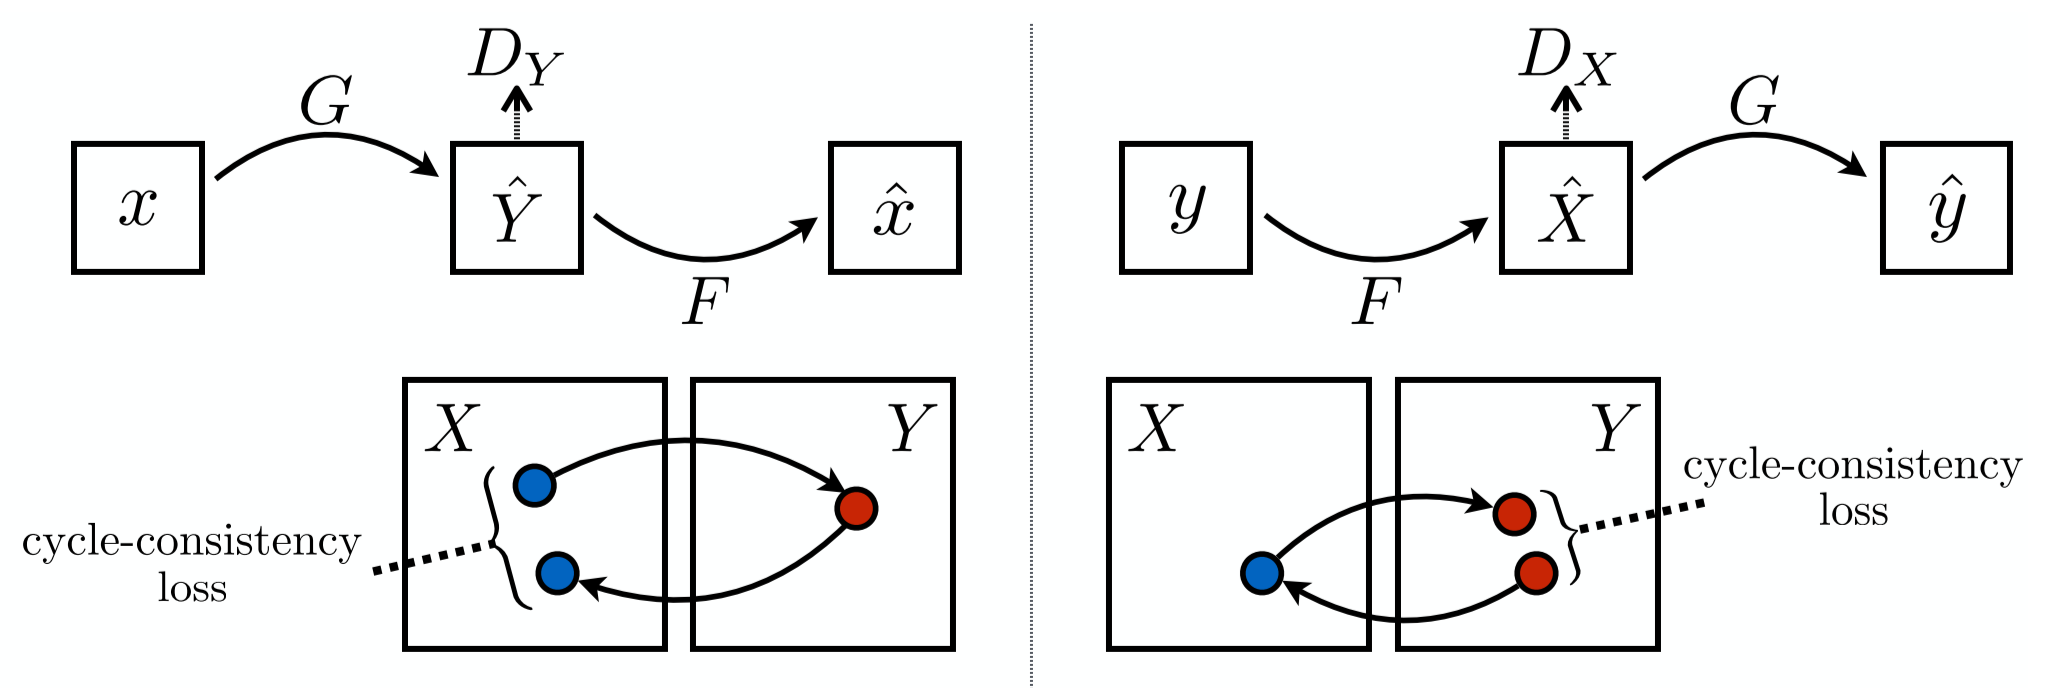
\includegraphics[width=\linewidth]{cycleConsistencyLoss}
	\caption{Cycle Consistency Losses in the back and forward translation~\cite{image-to-image-ccan}}
	\label{fig:cycleConsistencyLoss}
\end{figure*}


\subsection{Formulation}
In order to better understand the function and subsequent implementation of the losses, the mathematical background will be discussed in a bit more detail.

\paragraph{Adversarial Loss} is already used in training of standard \ac{GAN}s. It arises from the fact that the generator \textit{G} and discriminator \textit{D} work against each other. If the generator generates particularly good fake images that the discriminator can no longer identify as such, the loss of the discriminator automatically increases. On the other hand, the loss of the generator decreases. The loss behaviour is similar the other way round. This is described mathematically in \cite{Source-GAN} as follows:
\begin{equation*}
\begin{split}
\min_{G} \max_{D} V(D,G) =&~\mathbb E_{x \sim p_{data}(x)} [\log D(x)] \\\
&+ \mathbb E_{z \sim p_{z}(z)} [\log (1-D(G(z)))]
\end{split}
\end{equation*}

\paragraph{Cycle Consistency Loss} is used additionally to the adversarial loss in the Cycle-\ac{GAN}. The idea has already been briefly explained before, that a generator \textit{G} translates an image \textit{Input\_ A} from the domain \textit{X} into an image \textit{B} of the domain \textit{Y}. In the backward translation of generator \textit{F}, an image \textit{Cyclic\_ A} from domain \textit{X} will be created from the image \textit{B} of domain \textit{Y}. The difference between image \textit{Input\_ A} and \textit{Cyclic\_ A} forms the cycle consistency loss \cite{Introduction-to-Cycle-GANs}. In \cite{Introduction-to-Cycle-GANs}, the cycle consistency loss is described mathematically as follows:
\begin{equation*}
	Loss_{cyc}(G,F,X,Y) = \frac{1}{m} \sum^{m}_{i=1}[F(G(x_i))-x_i]+[G(F(y_i))-y_i]
\end{equation*}

In summary, the Cycle-\ac{GAN} is built from two generators, \textit{Generator A2B} and \textit{Generator B2A}, and two discriminators, \textit{Discriminator A} and \textit{Discriminator B}. This architecture is shown simplified in \autoref{fig:simplified-cycle-gan}.

\begin{figure}[htb] 
	\centering 
	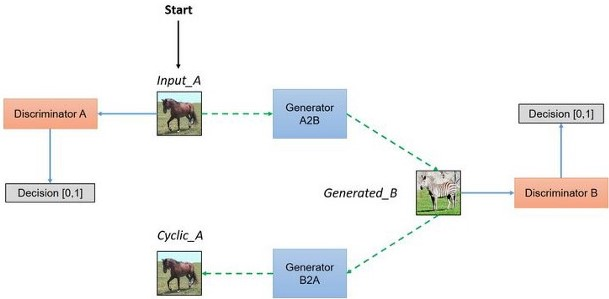
\includegraphics[width=\linewidth]{simplified-cycle-gan}
	\caption{A simplified architecture of a Cycle-\ac{GAN} \cite{Introduction-to-Cycle-GANs}}
	\label{fig:simplified-cycle-gan}
\end{figure}

\paragraph{Identity Loss} is also introduced in the paper \cite{image-to-image-ccan}. The loss is a regularization technology for the generator, to provide a better performs if the input is already near to the predicted output image. Mathematically the identity loss is defined in the paper \cite{image-to-image-ccan} as follows:
\begin{equation*}
\begin{split}
	Loss_{identity}(G,F) =&~\mathbb E_{y \sim p_{data}(y)}[||G(y) - y||_1] \\\
&+ \mathbb E_{x \sim p_{data}(x)}[||F(x)-x||_1]
\end{split}
\end{equation*}


\subsection{Datasets}
In addition to the architecture, a suitable datasets also had to be selected. On the one hand, it should be versatile, but on the other hand, it must not contain too large images so that the computing time is not too high. 

\paragraph{Tensorflow} provides different dataset specifically for Cycle-\ac{GAN}s including apple and orange images as well as photo and Monet images. These ones are called \textit{cycle\_gan/apple2orange} and \textit{cycle\_gan/monet2photo}. The datasets contain two domains A and B each for training and test data. \autoref{tab:dataset} shows the four parts of the default configuration with the number of examples included in each dataset. Each example consist of image-label pairs.~\cite{google-tf-datasets}

\begin{table}[htb]
\centering
\caption{Structure of the standard configuration split of the Tensorflow dataset \textit{cycle\_gan/apple2orange} and \textit{cycle\_gan/monet2photo}~\cite{google-tf-datasets}}
\label{tab:datasetTF}
\begin{tabular}{c c c}
\textbf{index} & \makecell[cc]{\textbf{examples} \\ \textbf{\texttt{apple2orange}}} & \makecell[cc]{\textbf{examples} \\ \textbf{\texttt{monet2photo}}}\\ \hline
'testA' & 266 & 121 \\ \hline
'testB' & 248 & 751 \\ \hline
'trainA' & 995 & 1072 \\ \hline
'trainB' & 1019 & 6287 \\ \hline
\end{tabular}
\end{table}

\paragraph{Kaggle} provides another dataset \textit{arnaud58/selfie2anime}. In order to make a further comparison, another dataset from a different library was deliberately selected. This one contains images of anime and images of women selfies. The examples included in this dataset are shown in \autoref{tab:datasetKaggle}. \cite{kaggle-dataset}

\begin{table}[htb]
\centering
\caption{Structure of the standard configuration split of the Kaggle dataset \textit{arnaud58/selfie2anime}~\cite{kaggle-dataset}}
\label{tab:datasetKaggle}
\begin{tabular}{c c}
\textbf{index} & \makecell{\textbf{examples} \\ \textbf{\texttt{selfie2anime}}} \\ \hline
'testA' & 100 \\ \hline
'testB' & 100 \\ \hline
'trainA' & 3400 \\ \hline
'trainB' & 3400 \\ \hline
\end{tabular}
\end{table}
%------------------------------------------------
\section{Implementation}
The implementation is performed using the learned three steps, pre-processing, training and test from the module \ac{IANNWTF} \cite{implementingANsCourseware02, implementingANsCourseware03}. In addition, the methods mentioned in the section before are used to develop the Cycle-\ac{GAN} architecture. Furthermore, other functions of the Tensorflow and Keras libraries are used in all parts of the implementation. Therefore, \texttt{tensorflow}, \texttt{tensorflow\_datasets}, \texttt{tensor- flow\_addons} and \texttt{matplotlib.pyplot} are imported. How the implementation is realized and the different libraries are used, is now explained in more detailed.

\subsection{Network Architecture}
The architecture is built as explained in section methods before. A class \texttt{Cycle\_GAN\_Generator} and a class \texttt{Cycle\_ GAN\_Discriminator} are programmed. Two instances of each of the two classes are then created, the \texttt{generator\_A \_to\_B} and \texttt{generator\_B\_to\_A}, and the \texttt{discriminator \_A} and \texttt{discriminator\_B}.

\paragraph{Generator Class} inherits from the Keras class \texttt{Layer}. The class in general is build up of three parts, the \textit{Encoder}, \textit{Transformer} and \textit{Decoder}. Each part consists again out of different layers. The structure of the generator is shown in \autoref{fig:generator}.~\cite{Introduction-to-Cycle-GANs}

\begin{figure*}[htb] 
	\centering 
	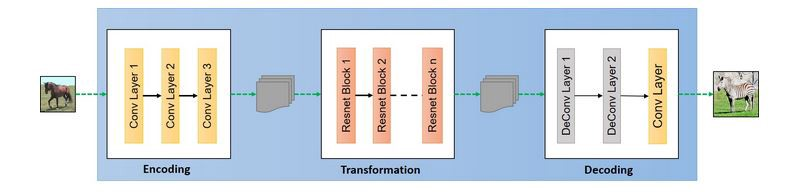
\includegraphics[width=\linewidth]{generator}
	\caption{The high-level structure of the Cycle-\ac{GAN}s generator \cite{Introduction-to-Cycle-GANs}}
	\label{fig:generator}
\end{figure*}

The \textbf{Encoder} extracts the feature of the original input image, for which convolutional layers are normally used \cite{Introduction-to-Cycle-GANs}. In \texttt{Cycle\_GAN\_Generator}, the encoder also consists of exactly three convolutional layers, as also described in \autoref{fig:generator}. The Keras class \texttt{Conv2D} is used for this. As activation function \ac{ReLu} is selected, for which the Keras class \texttt{ReLu} of the same name is used. Furthermore, the Keras class \texttt{InstanceNormalization} is used, which is a special form of group normalization, see \cite{google-tf-InstanceNormalization}, and is therefore suitable for the dataset used for the reimplementation. The normalization contains the argument axis, which is set to -1, which prevents the features per feature map from being normalized. So that the training does not exceed the time frame of the project, only a quarter of the original filter sizes of the paper are used in each \texttt{Conv2D} layer. All other values for \texttt{kernel\_size}, \texttt{strides}, \texttt{activation}, \texttt{padding} and the \texttt{kernel\_initializer} are taken identically from the specifications of the paper. The specifications and values for the three \texttt{Conv2D} layers are shown in \autoref{tab:encoderValues}.~\cite{image-to-image-ccan}

\begin{table}[htb]
\centering
\caption{Values of all convolutional layer specifications in the encoder part of the class \texttt{Cycle\_GAN\_Generator}~\cite{image-to-image-ccan}.}
\label{tab:encoderValues}
\begin{tabular}{c c c c}
\textbf{variable} & \makecell[cc]{\textbf{\texttt{Conv2D}} \\ \textbf{\texttt{Layer 1}}} & \makecell[cc]{\textbf{\texttt{Conv2D}} \\ \textbf{\texttt{Layer 2}}} & \makecell[cc]{\textbf{\texttt{Conv2D}} \\ \textbf{\texttt{Layer 3}}} \\ \hline
\textbf{\texttt{filters}} & 16 & 32 & 64 \\ \hline
\textbf{\texttt{kernel\_size}} & (7,7) & (3,3) & 3,3) \\ \hline
\textbf{\texttt{strides}} & (1,1) &  (2,2) & (2,2) \\ \hline
\textbf{\texttt{activation}} & None & None & None \\ \hline 
\textbf{\texttt{padding}} & "same" & "same" & "same" \\ \hline
\makecell[cc]{\textbf{\texttt{kernel\_}} \\ \textbf{\texttt{initializer}}} & \makecell[cc]{\texttt{Random} \\ \texttt{Normal}} & \makecell[cc]{\texttt{Random} \\ \texttt{Normal}} & \makecell[cc]{\texttt{Random} \\ \texttt{Normal}} \\ \hline
\end{tabular}
\end{table}

The \textbf{Transformer} is needed to relate closely spaced features extracted from the input image by the previous encoder \cite{Introduction-to-Cycle-GANs}. And this is exactly what the blocks of \acp{ResNet}, like shown in \autoref{fig:generator}, are needed for. Every \ac{ResNet} is build up by two \texttt{Conv2D} layers, two layers of \texttt{InstanceNormalization}, a \ac{ReLu} activation layer and a layer \texttt{Concatenate}, which is also a Keras class. A new class \texttt{ResNet\_Block}, which also inherits from the Keras class \texttt{Layer}, is implemented. All values for all layers are taken from the paper. The convolutional layer specifications are shown in \autoref{tab:transformerValues}.

\begin{table}[htb]
\centering
\caption{Values of the convolutional layer specifications in the transformer part of each \ac{ResNet} block of the class \texttt{ResNet\_Block}~\cite{image-to-image-ccan}.}
\label{tab:transformerValues}
\begin{tabular}{c c c}
\textbf{variable} & \makecell[cc]{\textbf{\texttt{Conv2D}} \\ \textbf{\texttt{Layer 1}}} & \makecell[cc]{\textbf{\texttt{Conv2D}} \\ \textbf{\texttt{Layer 2}}} \\ \hline
\textbf{\texttt{filters}} & 256 & 256 \\ \hline
\textbf{\texttt{kernel\_size}} & (3,3) & (3,3) \\ \hline
\textbf{\texttt{strides}} & (1,1) &  (1,1) \\ \hline
\textbf{\texttt{activation}} & None & None \\ \hline 
\textbf{\texttt{padding}} & "same" & "same" \\ \hline
\makecell[cc]{\textbf{\texttt{kernel\_}} \\ \textbf{\texttt{initializer}}} & \makecell[cc]{\texttt{Random} \\ \texttt{Normal}} & \makecell[cc]{\texttt{Random} \\ \texttt{Normal}} \\ \hline
\end{tabular}
\end{table}

Instances of this class are created as a layer in the class \texttt{Cycle\_GAN\_Generator}. The number of instances depends on the instance variable \texttt{n\_resnet}, which is set to six by default. Six \ac{ResNet} blocks are used if the image size is \textit{128~x~128}, nine blocks are use for an image size of \textit{256~x~256} or higher~\cite{image-to-image-ccan}.

The \textbf{Decoder} now leads back to an output image. For this, the low-level features are worked out with the help of the transpose convolution, see \cite{Introduction-to-Cycle-GANs}. To achieve this, the Keras class \texttt{Conv2DTranspose} is used in this part. Finally, as shown in \autoref{fig:generator}, another \texttt{Conv2D} is used, in conjunction with an activation function of the Keras class \texttt{tanh}. The values of the transposed convolution layer specifications is found in \autoref{tab:decoderValues1}, for the convolutional layer specifications in \autoref{tab:decoderValues2}.

\begin{table}[htb]
\centering
\caption{Values of the transposed convolutional layer specifications in the decoder part of the class \texttt{Cycle\_GAN\_Generator}~\cite{image-to-image-ccan}.}
\label{tab:decoderValues1}
\begin{tabular}{c c c}
\textbf{variable} & \makecell[cc]{\textbf{\texttt{Conv2D}} \\ \textbf{\texttt{Transpose}} \\ \textbf{\texttt{Layer 1}}} & \makecell[cc]{\textbf{\texttt{Conv2D}} \\ \textbf{\texttt{Transpose}} \\ \textbf{\texttt{Layer 2}}} \\ \hline
\textbf{\texttt{filters}} & 32 & 16 \\ \hline
\textbf{\texttt{kernel\_size}} & (3,3) & (3,3)  \\ \hline
\textbf{\texttt{strides}} & (2,2) & (2,2)  \\ \hline
\textbf{\texttt{activation}} & None & None  \\ \hline 
\textbf{\texttt{padding}} & "same" & "same" \\ \hline
\makecell[cc]{\textbf{\texttt{kernel\_}} \\ \textbf{\texttt{initializer}}} & \makecell[cc]{\texttt{Random} \\ \texttt{Normal}} & \makecell[cc]{\texttt{Random} \\ \texttt{Normal}}  \\ \hline
\end{tabular}
\end{table}

\begin{table}[htb]
\centering
\caption{Values of the convolutional layer specifications in the decoder part of the class \texttt{Cycle\_GAN\_Generator}~\cite{image-to-image-ccan}.}
\label{tab:decoderValues2}
\begin{tabular}{c c}
\textbf{variable} & \makecell[cc]{\textbf{\texttt{Conv2D}} \\ \textbf{\texttt{Layer 4}}} \\ \hline
\textbf{\texttt{filters}} & 3 \\ \hline
\textbf{\texttt{kernel\_size}} & (7,7) \\ \hline
\textbf{\texttt{strides}} & (1,1) \\ \hline
\textbf{\texttt{activation}} & None \\ \hline 
\textbf{\texttt{padding}} & "same" \\ \hline
\makecell[cc]{\textbf{\texttt{kernel\_}} \\ \textbf{\texttt{initializer}}} & \makecell[cc]{\texttt{Random} \\ \texttt{Normal}} \\ \hline
\end{tabular}
\end{table}

\paragraph{Discriminator Class} also inherits from the Keras class \texttt{La- yer}. In this reimplementation the class isn't a simple discriminator class, but a so called \textit{Patch\ac{GAN}}. This one is made up to not only output a single value, but a one-channel feature map of predictions. In this case the output refers to a \textit{70~x~70} receptive field of the original input. Since it has an image as input and a decision vector as output, \texttt{Conv2D} layers, are associated with \texttt{InstanceNormalization} and the activation function \texttt{LeakyReLu}. The values for the layers and there specifications are taken from the paper and are shown in \autoref{tab:discriminatorValues}. The original \texttt{filters} size here again is divided by four in the reimplementation to reduce training time. After first convolutional layer they didn't deliberately used \texttt{InstanceNormalization}. Last layer is a convolution to produce an output of 1-dimension. The structure of the discriminator is also shown in \autoref{fig:discriminator}. \cite{Introduction-to-Cycle-GANs}
\begin{table}[htb]
\centering
\caption{Values of the convolutional layer specifications in the discriminator class \texttt{Cycle\_GAN\_Discriminator}\cite{image-to-image-ccan}.}
\label{tab:discriminatorValues}
\begin{tabular}{c c c c}
\textbf{variable} & \makecell[cc]{\textbf{\texttt{Conv2D}} \\ \textbf{\texttt{Layer 1}}} & \makecell[cc]{\textbf{\texttt{Conv2D}} \\ \textbf{\texttt{Layer 2}}} & \makecell[cc]{\textbf{\texttt{Conv2D}} \\ \textbf{\texttt{Layer 3}}} \\ \hline
\textbf{\texttt{filters}} & 16 & 32 & 64 \\ \hline
\textbf{\texttt{kernel\_size}} & (4,4) & (4,4) & (4,4) \\ \hline
\textbf{\texttt{strides}} & (2,2) & (2,2) & (2,2) \\ \hline
\textbf{\texttt{activation}} & None & None & None\\ \hline 
\textbf{\texttt{padding}} & "same" & "same" & "same" \\ \hline
\makecell[cc]{\textbf{\texttt{kernel\_}} \\ \textbf{\texttt{initializer}}} & \makecell[cc]{\texttt{Random} \\ \texttt{Normal}} & \makecell[cc]{\texttt{Random} \\ \texttt{Normal}} & \makecell[cc]{\texttt{Random} \\ \texttt{Normal}} \\ \hline
\end{tabular}

\begin{tabular}{c c c}
\makecell[cc]{\\ \textbf{variable}} & \makecell[cc]{\\ \textbf{\texttt{Conv2D}} \\ \textbf{\texttt{Layer 4}}} & \makecell[cc]{\\ \textbf{\texttt{Conv2D}} \\ \textbf{\texttt{OutputLayer}}} \\ \hline
\textbf{\texttt{filters}} & 128 & 1 \\ \hline
\textbf{\texttt{kernel\_size}} & (4,4) & (4,4) \\ \hline
\textbf{\texttt{strides}} & (2,2) & (1,1) \\ \hline
\textbf{\texttt{activation}} & None & sigmoid \\ \hline 
\textbf{\texttt{padding}} & "same" & "same" \\ \hline
\makecell[cc]{\textbf{\texttt{kernel\_}} \\ \textbf{\texttt{initializer}}} & \makecell[cc]{\texttt{Random} \\ \texttt{Normal}} & \makecell[cc]{\texttt{Random} \\ \texttt{Normal}} \\ \hline
\end{tabular}
\end{table}

\begin{figure*}[htb] 
	\centering 
	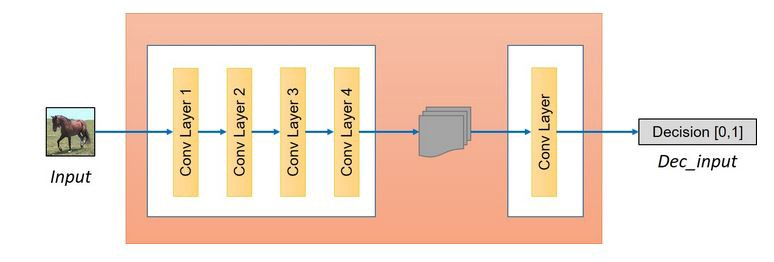
\includegraphics[width=0.8\linewidth]{discriminator}
	\caption{The high-level structure of the Cycle-\ac{GAN}s discriminator \cite{Introduction-to-Cycle-GANs}}
	\label{fig:discriminator}
\end{figure*}

\subsection{Pre-Processing}
In addition to creating the network architecture, the dataset must also be preprocessed. In order to implement easier switching between datasets and comparison versions, in addition to the reimplementation of the paper, different mechanisms were included. For switching between datasets, additional variables (\texttt{is\_selfie2anime\_dataset}, \texttt{is\_ap- ple2orange\_dataset}, \texttt{is\_monet2photo\_dataset}) were implemented to select the dataset to be pre-processed. At the beginning, these variables are used to select which dataset is to be loaded, by setting it \texttt{true}. Only one dataset can be loaded at a time. If several dataset arguments are set to true, the Kaggle dataset is preferred to the Tensorflow datasets due to the \texttt{if-elif-elif} query, and the \textit{apple2orange} dataset is preferred to the \textit{monet2photo} dataset.

Additionally, the dataset size is set to 900 training samples and 100 test samples after pre-processing to have a comparable number of images, between the different datasets. 

Moreover, since two different sources for the three datasets are used, there are a few different steps for pre-processing between the Tensorflow and Kaggle datasets. 

\paragraph{Tensorflow datasets} can be loaded more easily with the \texttt{tfds.load} function from the tensorflow library. In general there is more or less no difference between pre-processing \textit{cylce\_gan/apple2orange} or \textit{cylce\_gan/monet2photo} images. When the dataset is loaded, it is also directly split into test and training data, as well as in two domains for each, and requested as a 2-tuple structure (input, label). To ensure that all images are in the same format and that the training time is not too high, the images are subsequently resized to \textit{128~x~128}. After normalization to a value between $-1$ and $1$ ($2 * (img / 255) - 1$) and reshaping the tensor to \textit{128~x~128~x~3}, the dataset is shuffled and prefetched with a \texttt{buffer\_size} of 128. Batching is omitted, or rather set to one, to facilitate the later definition of real samples in training. All functions used are offered by the Tensorflow library. The values for arguments of the different pre-processing steps are taken directly from the paper.~\cite{image-to-image-ccan}

\paragraph{Kaggle datasets} need a few more pre-processing steps, than Tensorflow ones. The dataset \textit{arnaud58/selfie2anime} is downloaded with Keras function \texttt{image\_dataset\_from\_ directory} and directly batched to one. Because the dataset comes up as one big file, in which the dataset is separated in the different classes mentioned in \autoref{tab:datasetKaggle}, see \cite{kaggle-dataset}, it then needs to be split manually. This is done by using the functions \texttt{take} and \texttt{skip}. Thereupon, the same steps are carried out as for the Tensorflow datasets mentioned before.


\subsection{Training}
Three training epochs are chosen with each epoch having 900 training steps. With these numbers, the training can still be done in a reasonable amount of time. To make the training clearer, various functions have been programmed for different steps in the execution of the program.
 
In the first step the generators are trained. The training starts with taking an image-label pair from domain A and from domain B with the help of the function \texttt{generate\_real\_ dataset}. These pairs are randomly taken from the domains again for each training step. Afterwards the training for the \texttt{generator\_A\_to\_B} takes place and then for the generator \texttt{generator\_B\_to\_A}. Here for, the function \texttt{generator\_train\_step} was programmed, in which the adversarial loss (\texttt{adv\_loss}), the identity loss (\texttt{id\_loss}), the cycle consistency loss for the forward (\texttt{for\_loss}) and backward cycle (\texttt{back\_loss}) and the entire training loss (\texttt{train\_loss}) is computed. The training loss is composed of all other losses as follows:
\begin{equation*}
\begin{split}
train\_loss = &~(1 * adv\_loss) \\
&+ (10 * (for\_loss + back\_loss)) \\
&+ (5 * id\_loss)
\end{split}
\end{equation*}
In the papers implementation the identity loss is only used for the dataset \textit{cylce\_gan/monet2photo}. For better comparability between the different datasets, this was used to calculate the training loss in the reimplementation for all datasets. The training loss is then used in this function to update the generator parameters. To update the gradients of the generators, the loss function \textit{MeanAbsoluteError} is used. To update the generator parameters the optimizer \textit{Adam} is used.~\cite{image-to-image-ccan, google-Adam, google-GradientTape}

In the second step of each training step, the discriminators are trained. Since the discriminator is to identify the output image of the generator, the image from the selected image-label pair of domains A and B is fed to the respective generator before training and the result image is returned (function: \texttt{generate\_fake\_dataset}). However, the discriminator is now not simply passed this training image. This image is now stored in a history buffer. The function \texttt{update\_image\_pool} stores the image in the buffer and returns it at the same time, if the pool is not yet filled with 50 images. As soon as the pool is filled with 50 images, a random image from the buffer is exchanged against the current training image when the function is called. The exchanged image is then given to the discriminator as input. So it can happen that the discriminator gets an image, where it is easier for the discriminator to distinguish a generated image from a real image, because the image was generated by a worse generator version. This prevents, after \cite{oscillation}, the oscillation of \ac{GAN}s. With the passed image a forward step is performed and the loss is calculated as \textit{MeanSquaredError}. The loss is divided by two when updating the gradients to reduce the learning rate of the discriminator. The parameter update is also performed with the Optimizer Adam.~\cite{image-to-image-ccan, google-Adam, google-GradientTape}

To be able to document the training progress, the losses are averaged over the last 150 training steps and saved in a list. At the end of the program, these lists are saved in an Excel spreadsheet in Google Drive. The evaluation is then carried out with these values from these lists.

\subsection{Test}
As in the training, this time image-label pairs are taken from the test datasets of domain A and domain B. The image-label pairs are then used to generate the test data. Subsequently, the \texttt{generator\_test\_step} and \texttt{discriminator\_test\_step} functions calculate all the different losses, as in the training. However, this time parameters of the generators and discriminators are not updated. The losses are only returned for tracking.
For the representation and storage of the results further functions were programmed in addition to the reimplementation. Like mentioned before, also the test losses are saved into Excel files in the Google Drive. After 300 training steps a test is conducted. Each test phase conducts 100 steps. The losses are averaged over these 100 test steps and saved. Moreover, the test and training losses are displayed in the notebook every 450 training steps, so two times per epoch. Additionally, five images are selected from the test dataset for the training at the beginning, which are fed to Cycle\ac{GAN} in each test, i.e. three times per epoch. The original images and the images generated from them are stored in a Google Drive folder structure. This ensures a better comparability between the different ones after different training periods. The folder structure is built up as shown in \autoref{fig:fileStructure}.

\begin{figure}[htb] 
	\centering 
	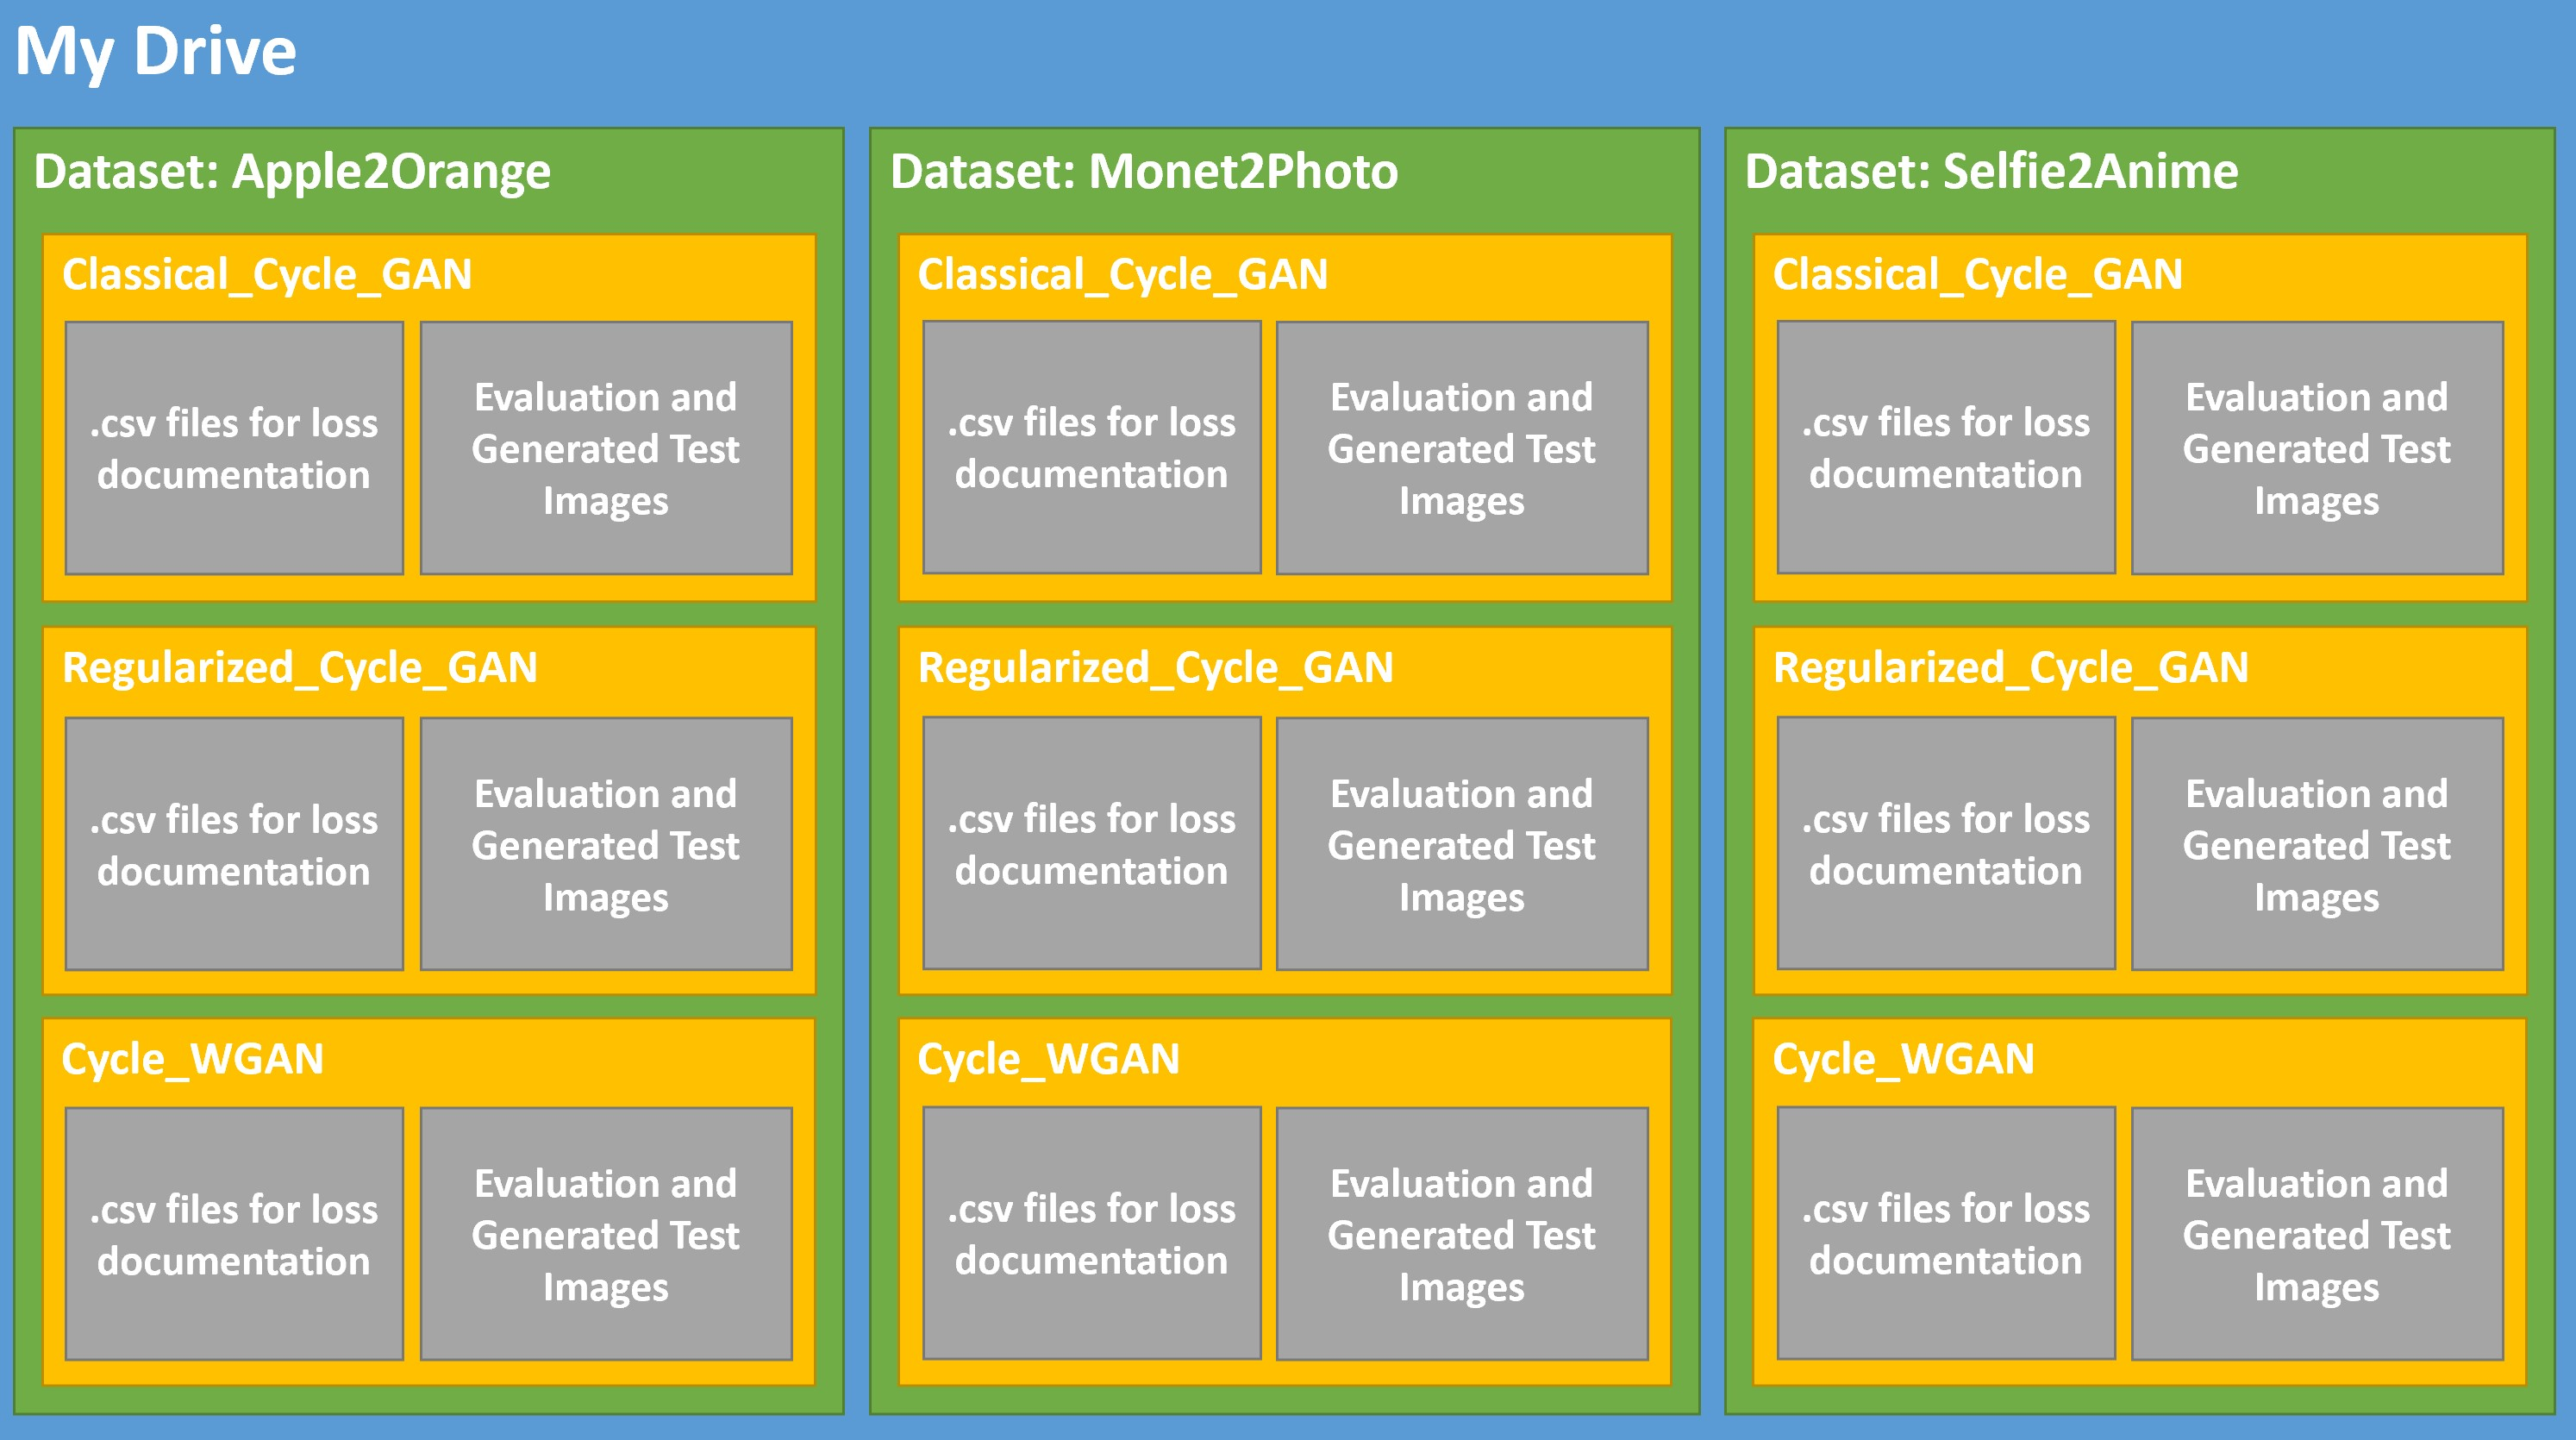
\includegraphics[width=\linewidth]{fileStructure}
	\caption{The folder structure of storing data in the Google Drive from the Colab script.}
	\label{fig:fileStructure}
\end{figure}

%------------------------------------------------
\section{Evaluation}
After the pure reimplementation of the Cycle-\ac{GAN}, two further improvements are implemented. All three variants are then compared with each other. The implementation of the two improved variants is explained in more detail in the following two subsections.

\subsection{Regularized \ac{ResNet} Blocks}
The first idea is taken from the original paper, see \cite{image-to-image-ccan}, and continued. Here also the Cycle-\ac{GAN} was already tested with options for the regularization. In this variant a further class for the \ac{ResNet} block, the \texttt{Regularized\_ResNet\_Block}, was programmed. This contains additionally a dropout layer, after the first convolutional layer. The dropout rate is assumed to be $0.5$.

Since the code should be written lean and collected in one colab notebook, the generator class is passed another argument at initialization, the \texttt{Regularized\_Cycle\_GAN}. If this argument is set to \textit{false}, then the default \ac{ResNet} is used during initialization. Is this argument set to \textit{true} during initialization, the Cycle-\ac{GAN} is built with regularized \ac{ResNet} blocks.

Beside the adjustment of the \ac{ResNet} blocks in the generator also the discriminator is adjusted. Already when initializing an instant of the discriminator class the argument \texttt{kernel\_regularizer} with a L2 loss regularizer is introduced with the convolutional layers. In the standard version of the Cycle-\ac{GAN} this is also initialized, but not used. In the training and test therefore also an argument, \texttt{Regularized\_ Cycle\_GAN}, is used, in order to control the computation of the loss dependent on it. If the argument is set to \textit{true}, the L2 loss for the discriminator is calculated and used for parameter adjustment.


\subsection{Cycle Wasserstein\ac{GAN}}
Furthermore, another method is introduced, according to \cite{wgan-improvement}. Here, instead of proceeding according to a simple \ac{GAN}, this is replaced by a \ac{WGAN}. This leads to the fact that first of all instead of the optimizer \textit{Adam}, the optimizer \textit{\ac{RMSProp}} is used. In addition, the weights in the discriminator are clipped, which also leads to the fact that the discriminator now has to be trained five times more than the generator. Furthermore, the \textit{sigmoid} activation is removed from the output layer of the discriminator. To implement all of this, a new class, \texttt{Cycle\_WGAN\_Discriminator}, is programmed for the \ac{WGAN} discriminator.

So that the network can also be included in the same lean colab notebook, the argument \texttt{Cycle\_WGAN} is introduced. If the argument is set to \textit{true}, then a Cycle-\ac{WGAN} is created, in the other case a standard Cycle-\ac{GAN}. Here then also the optimizer is initialized instead of as \textit{Adam}, as \textit{\ac{RMSProp}}.

%------------------------------------------------

\section{Results}

\subsection{Training vs. Test}
\begin{enumerate}[noitemsep] % [noitemsep] removes whitespace between the items for a compact look
	\item Welche Ergebnisse erzielt das Training?
	\item Welches Ergebnis erzielt der Test?
\end{enumerate}

\subsection{Comparison of datasets}
\begin{enumerate}[noitemsep] % [noitemsep] removes whitespace between the items for a compact look
	\item Welche Ergebnisse erzielt apple2orange?
	\item Welche Ergebnisse erzielt monet2photo?
	\item Welche Ergebnisse erzielt selfie2anime?
	\item Welche Ergebnisse zielen sie im vergleich zu einander?
\end{enumerate}

\subsection{Comparison of network variations}
\begin{enumerate}[noitemsep] % [noitemsep] removes whitespace between the items for a compact look
	\item Welche Ergebnisse erzielt standard cycleGAN?
	\item Welche Ergebnisse erzielt regularized cycle GAN?
	\item Welche Ergebnisse erzielt wasserstein cycle gan?
	\item Welche Ergebnisse zielen sie im vergleich zu einander?
\end{enumerate}

%------------------------------------------------

\section{Limitations and Discussion}

\begin{enumerate}[noitemsep] % [noitemsep] removes whitespace between the items for a compact look
	\item Datensatz/Bildgröße
	\item Dauer des Trainings und beanspruchung der rechenzeit
	\item noch besser wäre es wenn die 5 bilder noch zwischen den Unterschiedlichen GAN varianten gleich wäre, aber auf grund von shuffel ist das nicht so einfach und da das notepad immer neu gestartet wird
	\item besser test und training gleichviele abspeichern oder noch öfter, aber das wäre zu zeit intensiv
\end{enumerate}

%----------------------------------------------------------------------------------------
%	REFERENCE LIST
%----------------------------------------------------------------------------------------

\phantomsection
\bibliographystyle{unsrt}
\bibliography{sample}

%----------------------------------------------------------------------------------------

\begin{acronym}
\acro{BAIR}[BAIR]{Berkeley AI Research}
\acro{IANNWTF}[IANNWTF]{Implementing Artificial Networks with Tensorflow}
\acro{GAN}[GAN]{Generative Adversarial Network}
\acro{ReLu}[ReLu]{Rectified Linear Units}
\acro{ResNet}[ResNet]{Residual Network}
\acroplural{ResNet}[ResNet]{Residual Networks}
\acro{RMSProp}[RMSProp]{Root Mean Squared Propagation}
\acro{WGAN}[WGAN]{Wasserstein \ac{GAN}}
%\acroplural{Kuerzel}[Kurzform des Plurals]{Langform des Plurals}
\end{acronym}

%----------------------------------------------------------------------------------------


\end{document}